\begin{figure}
    \centering
    \begin{subfigure}[b]{0.32\textwidth}
        \centering
        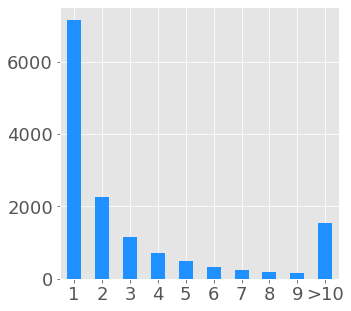
\includegraphics[width=\textwidth]{images/hist_words_freq_grouped_gt10.png}
        \caption{}
        \label{subfig:hist_word_freq}
    \end{subfigure}
    \hfill
    \begin{subfigure}[b]{0.32\textwidth}
        \centering
        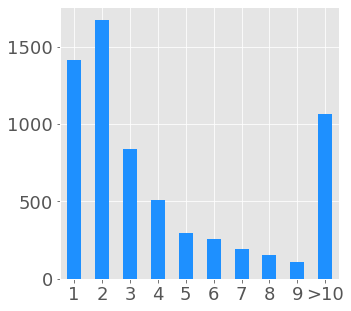
\includegraphics[width=\textwidth]{images/hist_words_freq_no_sing_grouped_gt10.png}
        \caption{}
        \label{subfig:hist_words_freq_no_sing}
    \end{subfigure}
    \hfill
    \begin{subfigure}[b]{0.32\textwidth}
        \centering
        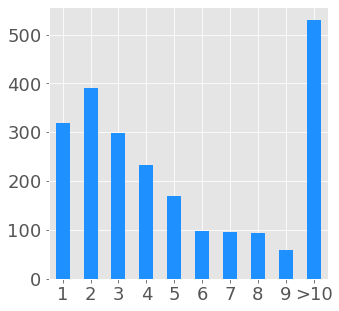
\includegraphics[width=\textwidth]{images/hist_words_freq_no_lt5_grouped_gt10.png}
        \caption{}
        \label{subfig:hist_words_freq_no_lt5}
    \end{subfigure}
    \caption{Histograms of word frequency over the whole dataset (a), after removing samples with singletons (b) and and after removing samples with words with frequency lower than 5 (c).}
    \label{fig:words_statistics}
\end{figure}